\documentclass{report}
\usepackage{cite}
\usepackage{titlesec}
\usepackage{amsmath}
\usepackage[english]{babel}
\usepackage{caption}
\usepackage{multirow}
\usepackage{tikz}
\usepackage{amsmath}
\usepackage{amssymb}
\usetikzlibrary{calc}
\usetikzlibrary{arrows}
\usepackage{pgfplots}
\captionsetup[figure]{font=small}	
\captionsetup[table]{font=footnotesize}
\newcommand{\R}{\mathbb{R}}
\usepackage{float}
\tolerance=1
\emergencystretch=\maxdimen
\hyphenpenalty=10000
\hbadness=10000
\usepackage{array}
\usepackage[margin=1.5in]{geometry}
\usepackage{mathtools}

\begin{document}


\begin{titlepage}
\begin{center}
\vspace*{0.8cm}
\begin{figure}[H]
\centering

\includegraphics[width=0.4\textwidth]{logo_uni}
\end{figure}
\LARGE{\textsc{University of Padua}}\\
\vspace*{0.1cm}
\Large{\textsc{Department of Information Engineering}}\\
\vspace*{1.8cm}
\Large{\textsc{Information Security Report}}\\
\vspace*{0.1cm}
\Large{\textsc{Team Maracas}}\\
\vspace*{0.8cm}
\huge{\textbf{Implementation of random binning encoding and secrecy rate evaluation 
}}\\
\vspace*{1cm}
\end{center}
\large{\textit{Authors:}}
\hfill
\large{\textit{Teacher:}} \\
\large{Lejla \textsc{D\v{z}anko}}
\hfill
\large{Nicola \textsc{Laurenti}}\\
\large{Simone \textsc{Favaro}}\\
\large{Davide \textsc{Frizzo}}\\
\large{Claudio \textsc{Stefani}}\\
\large{Edoardo \textsc{Trombin}}\\

\begin{center}
\large{28th November 2020}\\
\end{center}
\end{titlepage}
\pagebreak




\setcounter{page}{1}
\pagenumbering{arabic}




\begingroup
\let\clearpage\relax
\chapter*{Abstract}
\endgroup
The aim of this Laboratory Session is to analyse Physical Layer Secrecy mechanisms and to study their performances. In particular, we will analyse a random binning encoder and decoder in two different situations. First, we will consider a uniform error channel connecting the encoder and the decoder, and then a BSC (Binary Symmetric Channel). The implementations of all the solutions and considerations expressed in this report are done using the Python programming language. 





\begingroup
\let\clearpage\relax
\chapter*{General settings}
\endgroup
\begin{itemize}
\item All the mechanisms work in the binary field $\sum = \{0,1\}$ 
\item The secret message is a 3 bit message $M=\{0,1\}^3$ 
\item The messages used by the encoder, the channel and the decoder are 7 bit messages $X=Y=Z=\{0,1\}^7$
\item The output $y$ and $z$ of the channel are conditionally uniform and independent of each other given  $x$. 
\end{itemize}




\chapter*{Task implementation}
\section*{Task 1 - Implement the uniform error channel}
The uniform error channel takes as input a message $x\in X$ (that will be the output of the encoder) and returns as output $y\in Y$ in the legitimate channel $A\to B$ and $z\in Z$ in the illegitimate channel $A\to E$.  As the name suggests this channel extracts uniformly at random the output from the set of all possible outputs, given a certain input $x\in X$. 

\subsection*{Legitimate channel A $\boldsymbol{\to}$ B:}
The legitimate channel introduces at most 1 error per word. Given an input $a\in X$ let the set of all the possible outputs of the channel be $T_{y|x}(a)$. This set contains all the elements in $Y$ that have Hamming distance at most 1 from $a$. These elements are 7-bit zero binary numbers (in case of 0 errors), plus the 7-bit binary numbers with Hamming distance equal to 1 w.r.t. $a$ (they can be computed XORing the input a with all 7-bit binary numbers with Hamming distance equal to 1 w.r.t. the 7-bit 0 vector). There are 7 of them, so the set $T_{y|x}(a)$ contains 1+7 elements: 
\begin{equation*}
\begin{aligned}
T_{y|x}(a)= \{b\in Y : dH(a, b)\leq1\} = a\oplus \{0000000, 0000001, 0000010, 0000100, 0001000, 0010000,\\ 0100000, 1000000\}
\end{aligned}
\end{equation*}


\subsection*{Illegitimate channel A $\boldsymbol{\to}$ E:}
This channel introduces at most 3 errors per word. So, given a certain input $a\in X$ the set of all  possible output $T_{y|z}(a)$ contains all the elements in $Y$ that have Hamming distance at most 3  from $a$. Following the reasoning used before, these elements are 7-bit zero binary numbers in case of 0 errors, the 7-bit  binary numbers with Hamming distance equal to 1 w.r.t. the 7-bit 0 vector (which are 7) in case of 1 error, the 7- bit binary numbers with Hamming distance 2 (which are 21) in case of 2 errors and the 7-bit  binary numbers with Hamming distance equal to 3 (which are 35) in case of 3 errors, for a total of  64 numbers: 
\begin{equation*}
Tz|x(a) = \{c\in Z : dH(a, c)\leq3\} = a\oplus \{0000000, 0000001, ..., 1101000, 111000\}
\end{equation*}
To verify the uniformity of the channel we simulate $10^4$ realizations of the channel with the same  input $x$=1001000 to compute the conditional pmd $P_{z|x}(\cdot |1001000)$. To compute the probability of $a$ particular $z\in Z$ we: 
\begin{itemize}
\item store all the $10^4$ values of $z$ obtained from the realizations in a matrix $Z$;
\item for each possible value that $z$ could take (all the integers between 0 and 127) count how many  occurences of that value are contained in $Z$ and compute the probability dividing by $10^4$ 
\end{itemize}
After collecting the conditional probability for each of the possible $z\in Z$ it’s possible to realize a  plot of the conditional pmd $P_{z|x}(\cdot|1001000)$:

\begin{figure}[H]
\centering
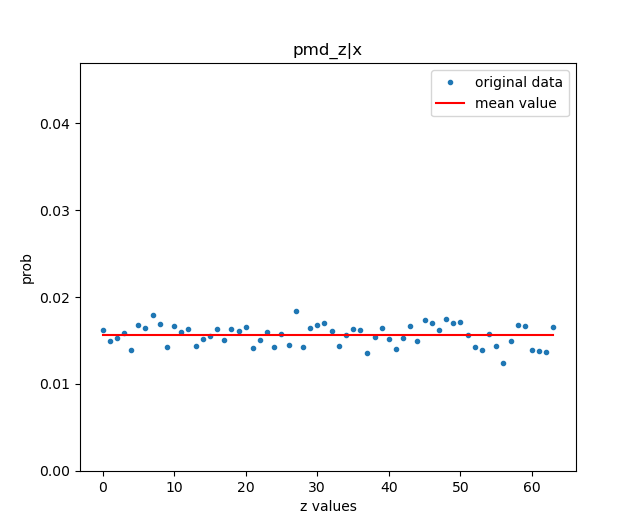
\includegraphics[width=0.8\textwidth]{plot1}
\end{figure}

Since the illegitimate channel introduces no more than 3 errors it’s not possible to obtain values of $z$ with Hamming distance greater than 3 from the input $x$=1001000 (so for example it’s not possible to obtain $z$=1111111). That’s why in the plot there are some missing values. Looking at the occurring values (the ones with Hamming distance from $z$ less or equal than 3), they have almost the same probability and the plot is approximately similar to the one of the PMD  of a Uniform random variable (increasing the number of iterations makes it even more visible). 




\section*{Task 2 - Implement the random binning encoder}
We implemented a random binning encoder where: 
\begin{itemize}
\item the code used is the (7,4) Hamming code: 
\begin{equation*}
\begin{aligned}
X’= \{0000000, 1000110, 0100101, 0010011, 0001111, 1100011, 1010101, 1001001,  0110110, 0101010,\\
0011100, 1110000, 1101100, 1011010, 0111001, 1111111\}
\end{aligned}
\end{equation*}
\item the set of all possible codewords associated to a given input $d\in M$ $T_{x|u}(d)$ is made of 2  codewords: the first one has a 4 bit prefix [0,d], the second one is the binary complement of the first codeword. As there are 8 possible values for the secret message $d\in M$ and 2 possible codewords connected to it, all the output space $X’$, that is composed of 16 codewords, is covered. 
\end{itemize}




\section*{Task 3-Implement the random binning decoder}
The decoder takes as input the output of the channel $y\in Y$. Since the channel introduces some errors it’s possible that the received word $y$ is different from the word $x$ transmitted from the encoder. To retrieve the original $x$ we use the minimum Hamming distance criterion, choosing as $\hat{x}$ the codeword in $X’$ that has the minimum Hamming distance from $y$. Once we obtained $\hat{x}$, to identify the transmitted message $\hat{u}$ we just have to look at the first bit of $\hat{x}$: 
\begin{itemize}
\item if the first bit is equal to 0 than the codeword transmitted is the first of the pair given by $T_{x|u}(\hat{u})$ so we return the bits 2-4 of $\hat{x}$. 
\item if the first bit is equal to 1 then the codeword transmitted is the second of the pair so we return the binary complement of the bits 2-4 of $\hat{x}$. 
\end{itemize}
It’s possible to verify the correctness of our implementation observing the output of the cascade  encoder$\to$decoder where the initial input message $u$ is correctly decoded $(\hat{u}=u)$. The same for the  cascade encoder$\to$legitimate channel$\to$decoder that works because of the property of the Hamming code to correct the (at most) 1 error per word introduced by the channel. 




\section*{Task 4 - Verify perfect secrecy}
To verify the perfect secrecy of the wiretap channel, we must show that the illegitimate channel output $z$ is independent from the secret message $u$. In order to do so it’s possible to look at the mutual information between $u$ and $z$, $I(u,z)$. This quantity in fact is equal to the \textit{Kullback-Leibler Divergence}(KLD) between the joint pmd $P(u,z)$ and its independent counterpart $P(u)\cdot P(z)$. So the mutual information can be seen as a measure of how far $u$ and $z$ are from being independent. In case of independence in fact the mutual information is equal to 0.\\
The formula to compute the mutual information is the following: 
\begin{equation*}
I(u,z)=\sum_{d\in M, c\in Z}p_{u,z}(d,c)\cdot log_2\frac{p_{u,z}(d,c)}{p_u(d)\cdot p_z(c)}
\end{equation*}
To compute the mutual information we first need to compute all the different PMDs. The starting  point is the computation of the conditional PMD $P[z|u]$: for each possible value of the input  message $u$ we do 10000 simulations of the chain encoder + illegitimate channel and collect the outputs $z$ obtained. For each possible value of $z$ we estimate its conditional probability given a certain $u$ dividing the number of occurrences we get for $z$ by 10000.\\
Assuming that the distribution of the message $u$ is uniform over the message space $M$ it’s possible to compute the other PMD using the following formulas:
\begin{equation*}
P[u=u',z=z']=P[z=z'|u=u']\cdot P[u=u']
\end{equation*}
\begin{equation*}
P[z=z']=\sum_{u'\in M}P[u=u',z=z']
\end{equation*}
Finally we can compute the mutual information that turns out to be equal to:
\begin{equation*}
I(u,z)=0.0072
\end{equation*}
This result shows that the messages $u$ and $z$ are (almost) empirically independent since the value of the mutual information is near to 0.\\
We can finally draw the plot of $P[z|u]$ and of $P[z]$ (we are showing just one of the 8 different conditional distributions obtainable, the rest are present in the Python code): 

\begin{figure}[H]
\centering
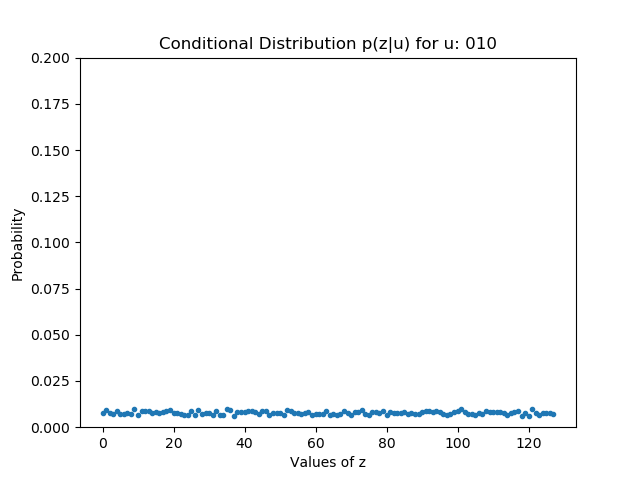
\includegraphics[width=0.8\textwidth]{plot6}
\end{figure}

\begin{figure}[H]
\centering
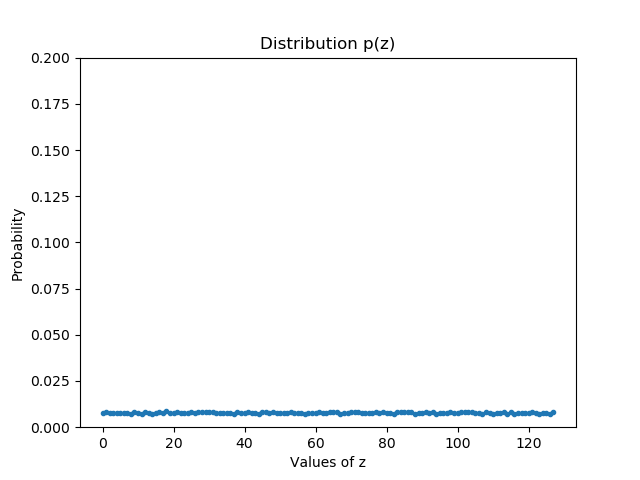
\includegraphics[width=0.8\textwidth]{plot7}
\end{figure}

Since $u$ and $z$ are independent the knowledge of $u$ should not add any information to the uncertainty of $z$, in fact the two plots are very similar.

\subsection*{Considerations and Remarks}
Answers to the questions in slide 16: 
\begin{enumerate}
\item We verified that the wiretap channel implemented achieves both perfect reliability and perfect
secrecy:
\begin{itemize}
\item perfect reliability: $|X'|\leq \frac{|Y|}{N_{y|x}}$
\item perfect secrecy: $|N_{x|u}|\geq \frac{|Z|}{N_{z|x}}$
\item so, to achieve both perfect reliability and perfect secrecy: $M=|M|\leq \frac{|X'|}{N_{x|u}}\leq \frac{|Y|}{N_{y|x}}\cdot\frac{N_{z|x}}{|Z|}=8$
\end{itemize}
So the number of secret bits per channel used is $log_2M = 3$ bits. This depends on how we use the code $X’$ in the encoder. In fact the Hamming code (7,4) is a linear block systematic code that has 4 information bits (the most 4 significant bits) in each codeword and the remaining 3 bits are redundant bits that are computed as a function of the information bits. So the number of independent bits, unpredictable for $E$, are actually 4 but in the definition of our encoder we set the first bit of the codeword equal to 0 (if the codeword chosen is the first) or equal to 1 (in the other case) so we are actually using 3 secret bits.\\
\item To have 4 secret bits we should use a 4-bit input message, so there are 16 possible values for $u$.  Using the same Hamming (7,4) code our encoder will be a one to one function since there is only 1  possible codeword associated with a certain message $u$, so it’s not possible to achieve 4 secret bits  with this wiretap channel settings. This is also apparent from the fact that the one to one map would bring $N_{y|x}=1$, and the previous inequality would not hold anymore. A possible solution could be achieved by using a different Hamming code with an increased block length (for example Hamming(15,11)). 
\item To have 2 secret bits we can change the implementation of the encoder in this way:
\begin{itemize}
\item we consider a 2 bit input message $u’$ (ex. $u’=00$)
\item we consider the two messages in $M$ with the 2-bit suffix equal to $u’$: $[0 + u’]$ and $[1 + u’]$ 
(ex. starting from u’ we get 000 and 100)
\item the message $u$ to be sent is chosen randomly and uniformly among these two and sent through the channel
\item the decoder simply computes the transmitted codeword implementing the minimum Hamming  distance criterion in the same fashion as before, and ends up considering just the two least significant bits of $u$, retrieving $u’$ 
\end{itemize}
In this new implementation we have the 2 secret bits because the most significant bit is basically ignored.
\item The Hamming (7,4) code always corrects an error but with 2 or more errors the result of the  minimum Hamming distance decoder is always wrong (since every binary word in our $\{0,1\}^7$ space is either a codeword or it’s at distance 1 from a codeword). So the only cases when Eve does not make an error in decoding is when the illegitimate channel introduces 0 or 1 error in the transmission of the codeword $x$, and this happens with a probability of: 
\begin{equation*}
\frac{\#error\_patterns\_with\_0\_or\_1\_error}{\#all\_possible\_error\_patterns}=\frac{8}{64}=\frac{1}{8}
\end{equation*}
So the only possibility for the eavesdropper is to randomly and uniformly guess each bit in the message to try to break the system.\\
Although we know that $\frac{1}{8}$ is the best we can achieve in terms of Eve’s success rate (uniformity over the message space $\{0,1\}^3$), an uninformed person could argue that $\frac{1}{8}$ is a very high success rate (it actually is, in general terms). However, the calculation of mutual information formally shows that we can’t do better, since a value very close to zero means that $u$ and $z$ are almost totally independent of each other.
\end{enumerate}




\section*{Task 5 - Simulate transmission over a binary symmetric channel (BSC)}
We now introduce a BSC channel with error rate $\varepsilon$ for the legitimate channel and $\delta$ for the  eavesdropper channel. To implement the BSC channel we used the Python \textit{bsc} function that, given as input parameters the input message and the channel error probability, returns the channel output.\\
Now we substitute the uniform error channel with the BSC channel between the encoder and the decoder in our transmission scheme to obtain a wiretap BSC channel. Feeding the encoder with different messages now the chain encoder$\to$BSC channel$\to$decoder is no more perfectly reliable as the one with the uniform error channel $(\hat{u}\neq u)$. This happens when the legitimate BSC channel has an error rate $\varepsilon$ such that more than 1 error is introduced. In this case the Hamming code is  able to correct only 1 of the errors so the decoded message $\hat{u}$ can be different from the original message $u$. 




\section*{Task 6 - Evaluate the system security over the wiretap BSC}
\subsection*{Evaluation of the system’s reliability}
To evaluate the reliability of the wiretap BSC we need to make realizations of the channel for several values of $\varepsilon$ and use the results obtained to estimate Bob’s error rate on the secret message $P[\hat{u} \neq u]$.\\
In order to do that: 
\begin{itemize}
\item for each pair $\varepsilon$ do 100 realizations of the wiretap BSC
\item in each realization collect the output $\hat{u}$ and compare it with the initial message
\item to compute $P[\hat{u}\neq u]$ for a particular pair $(\varepsilon, \delta)$ compute the division between the number of realizations in which $\hat{u}\neq u$ and the number of realizations done (100).
\end{itemize}
To analyse the result obtained it’s possible to draw a plot of $P[\hat{u}\neq u]$ as a function of $\varepsilon$:

\begin{figure}[H]
\centering
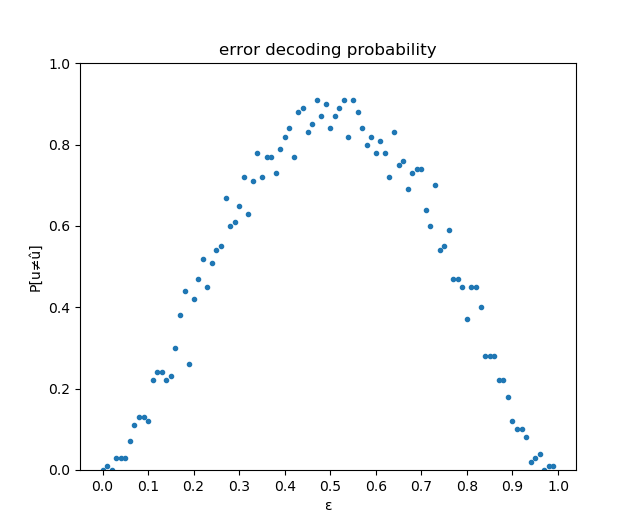
\includegraphics[width=0.7\textwidth]{plot2}
\end{figure}

As expected for values of $\varepsilon$ near 0 or to 1, the channel is almost perfect and the error rate  is approximately zero. On the other hand when $\varepsilon$ is near to 0.5 the channel is useless: every bit of the  input message has the same probability to be correct or to be flipped. In $\varepsilon=0.5$ the plot reaches its maximum value and $P[\hat{u}\neq u]$ is near to 1.\\
For the others values of $\varepsilon$: 
\begin{itemize}
\item as $\varepsilon$ increases from 0 to 0.5 the error rate increases
\item as $\varepsilon$ increases from 0.5 to 1 the error rate decreases
\end{itemize}

\subsection*{Evaluation of system’s secrecy}
In this part we evaluate the resulting secrecy in terms of leaked information to $E$ on the secret  message computing the mutual information between $u$ and $z$ $I(u,z)$. To compute the mutual information we use the same implementation used for task 4.\\
It’s now possible to compute the mutual information for the wiretap BSC for different values of the error rate $\delta$ in order to be able to draw a plot of $I(u,z)$ as a function of $\delta$: 

\begin{figure}[H]
\centering
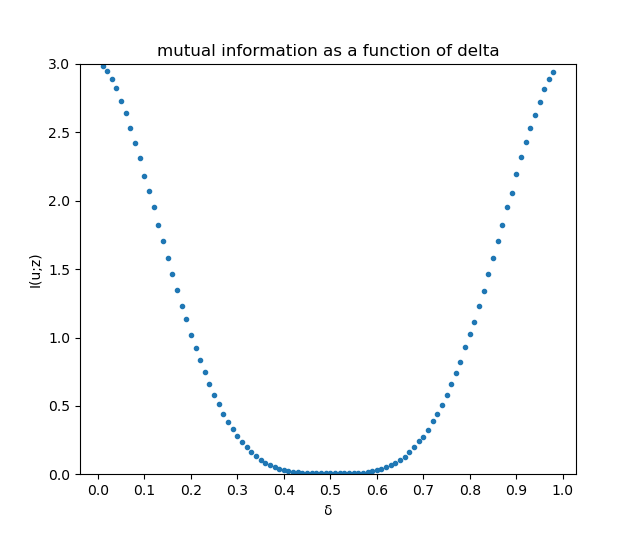
\includegraphics[width=0.7\textwidth]{plot3}
\end{figure}

Since the mutual information is a measure of the distance of how far $P(u,z)$ is from its independent  counterpart $P(u)\cdot P(z)$ when the error rate $\delta$ is near to 0.5, the BSC illegitimate channel is useless,  the message $u$ is independent to $z$ and the mutual information is near to 0. On the other hand, when $\delta$ is near to 0 or 1 the BSC illegitimate channel is almost perfect so the output $z$ has a high correlation with $u$ so the mutual information is high. In the extreme case of $\delta$ equal to 0 or 1 the eavesdropper is always able to retrieve u so the $I(u,z)=H(u)=log_2|M|=3$bit since we assume that the distribution of $u$ is uniform.\\
We finally draw a contour plot of the secrecy capacity of the mechanism as a function of $\varepsilon$ and $\delta$. The secrecy capacity of the BSC channel follows: 
\begin{equation*}
C_s=C_{AB}-C_{AE}=h_2{\varepsilon}-h_2(\delta)
\end{equation*}
Where:
\begin{equation*}
h_2(\varepsilon)=\varepsilon\cdot log_2\varepsilon + (1-\varepsilon)\cdot log_2(1-\varepsilon)
\end{equation*}
and similarly for $h_2(\delta)$.

\begin{figure}[H]
\centering
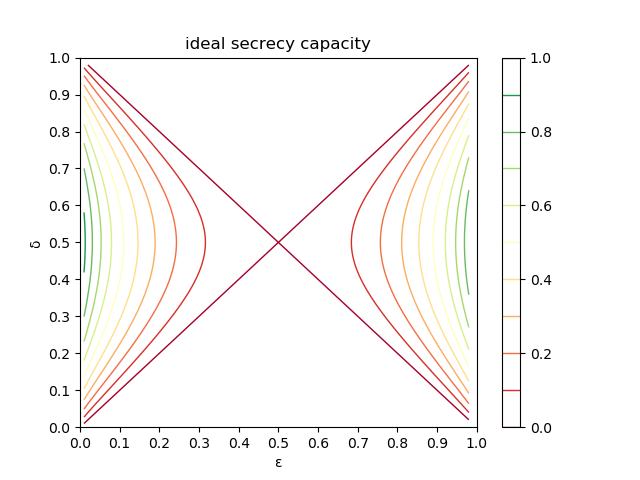
\includegraphics[width=0.8\textwidth]{plot4}
\end{figure}

\begin{figure}[H]
\centering
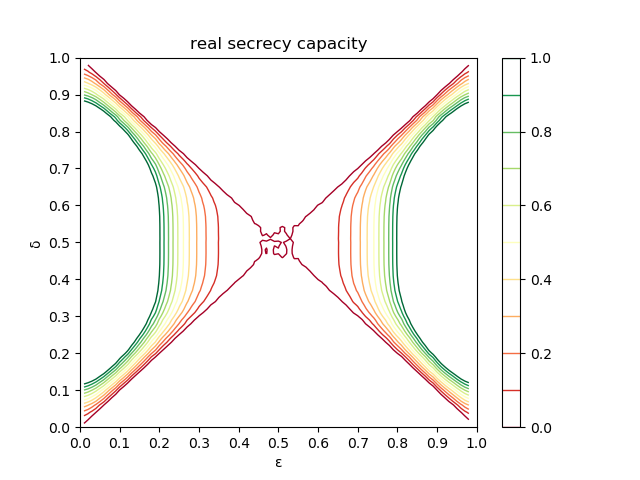
\includegraphics[width=0.8\textwidth]{plot5}
\end{figure}	

The first plot is the ideal one obtained with the Python function \textit{plt.contour} (it coincides with  the plot in slide 11 of the Instructions) while the second is the one obtained with our results. The two plots are really similar except for some noise in the right one.\\
The secrecy capacity is 0 when $\varepsilon$ is near 0.5 and $\delta$ is near to 0 or 1. Symmetrically the secrecy capacity is high when $\delta$ is near 0.5 and $\varepsilon$ is near to 0 or 1.




\end{document}

